\chapter{Simulation}
In unserer Arbeit haben wir eine Wissensbasis erstellt, welche Parameter inferrieren kann, womit ein Agent verschiedene Aktionen ausführen kann. Da es sich als herausfordernd darstellt die Aktionen auf einem realen Roboter zu testen tun wir dies in einer Simulation.
Dieses Kapitel soll einen Überblick über die Simulationsumgebung geben, in der wir unsere Arbeit testen und als Proof of Concept darstellen möchten.
Zunächst wollen wir die Umgebung, samt Objekten erläutern, darauf folgend möchten wir einen Überblick über die Motion Primitives geben.
Zum Schluss werden wir einige unserer Motions showcasen und über die SimToRealWorldGab sprechen, bevor wir einen Fazit ziehen, wo wir über vorhandene Schwierigkeiten diskutieren.

\section{Simulation Environment}
Wir benutzen die Simulationsumgebung BulletWorld \nameref{sec:pybullet}, welche sowieso in dem Framework PyCRAM \nameref{sec:pycram} genutzt wird. 
In dieser Umgebung wird die Physik dementsprechend auch simuliert, welches für die Ausführung der von uns definierten/angepassten Motions vorteilhaft ist.
Da wir außerdem das Framework \textit{PyCRAM} nutzen, ermöglicht sich uns die Möglichkeit der Benutzung verschiedener Control Primitiven, welche schon vorhanden sind, wie zum Beispiel Pick and Place.
Für die Kommunikation zwischen der Simulation und Framework wird ROS1 \nameref{sec:ROS} genutzt, welches über verschiedene Nodes kommuniziert, die jeweils zum Beispiel einen Joint repräsentieren.
Über diese Nodes kann man dementsprechend Informationen zu den Joints erhalten oder selbst Befehle übertragen, welche die Parameter der Joints dementsprechend verändern würden.

Der Agent, der in der Simulation die verschiedenen Motions ausführen wird, ist der PR2 \nameref{sec:pr2}. Dieses Robotermodell verfügt über 2 bewegbare Arme, dieser Aspekt ist wichtig für unsere Arbeit, da bei der Ausführung der Motions eine Hand die Motion ausführt, während der andere Arm den Container festhält, in dem die Aktion ausgeführt wird.
Neben der Tatsache, dass das Modell des PR2 schon im Framework PyCram vorhanden ist, verfügt das Modell des PR2's außerdem auch über genügend Joints und Degrees of Freedom, um die von uns angepassten Motions auszuführen.

Der Agent agiert in einer Küchenähnlichen Umgebung, dessen Modell auch im PyCRAM Core schon enthalten ist und dementsprechend sich auch für unseren UseCase besonders gut eignet. Die Küche verfügt auch über zum Beispiel Schubladen, welche geöffnet werden können, was zu einer Annaeherung an einer realen Küche hindeutet.
Das Modell der Küche verfügt außerdem über einen Tisch, worauf schlussendlich die Aktionen des Agenten ausgeführt werden.
Weitere Möbel sind auch in dieser Umgebung enthalten, diese sind allerdings für unseren Use Case nicht von Bedeutung.

\begin{figure}[H]
    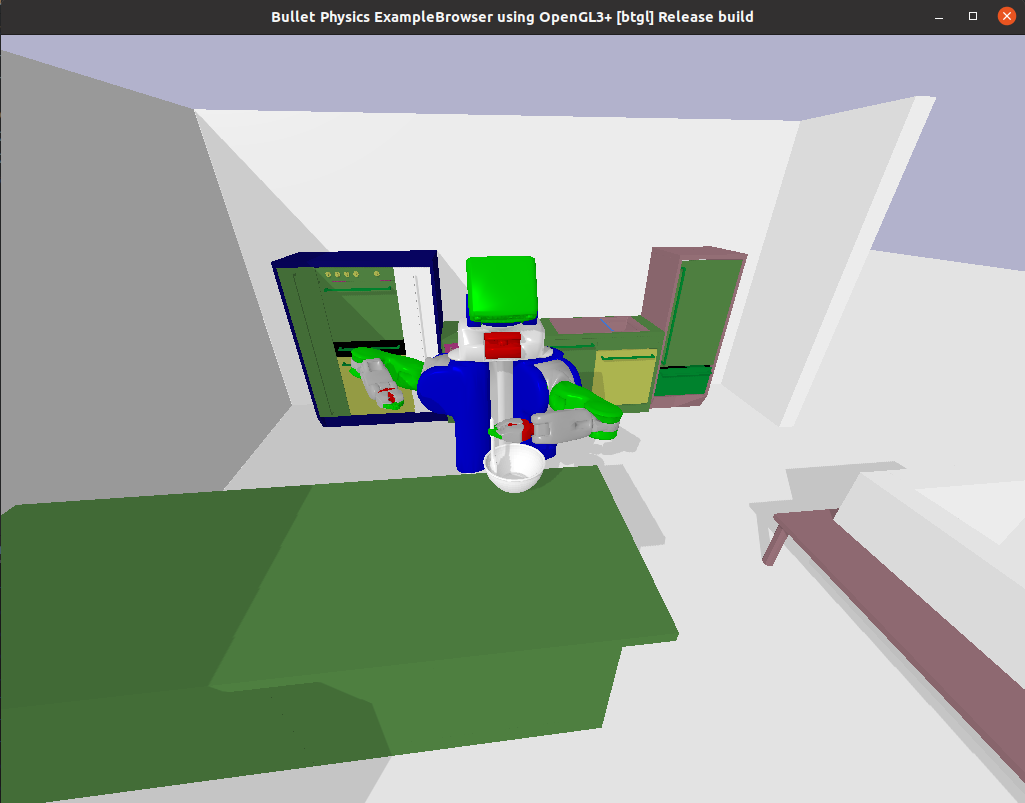
\includegraphics[scale=0.35]{Graphics/bulletworldexample.png}
    \label{fig:bulletworldexample}
    \caption{Simulation Environment containing the \textit{PR2} and \textit{Kitchen} models. }
\end{figure}

Für die Simulation nutzen wir die Objekte, welche auch in der Ontologie definiert wurden (siehe \nameref{sec:ContainersAndToolsAcquisition}).
Folgende Objekte sind vorhanden:
\begin{itemize}
	\item Container: kleine und große Bowl (in der Ontologie \textit{SaladBowl} und \textit{PastaBowl} definiert), Pfanne, Topf, Becher und Tasse.
	\item Tools: Whisk (auch wenn diese nicht in der Ontologie definiert wurde, nutzen wir sie trotzdem, da es doch ein sehr häufig vorkommnedes MixInstrument ist.), Löffel, Holzlöffel und Gabel. 
\end{itemize}

\begin{figure}[H]
    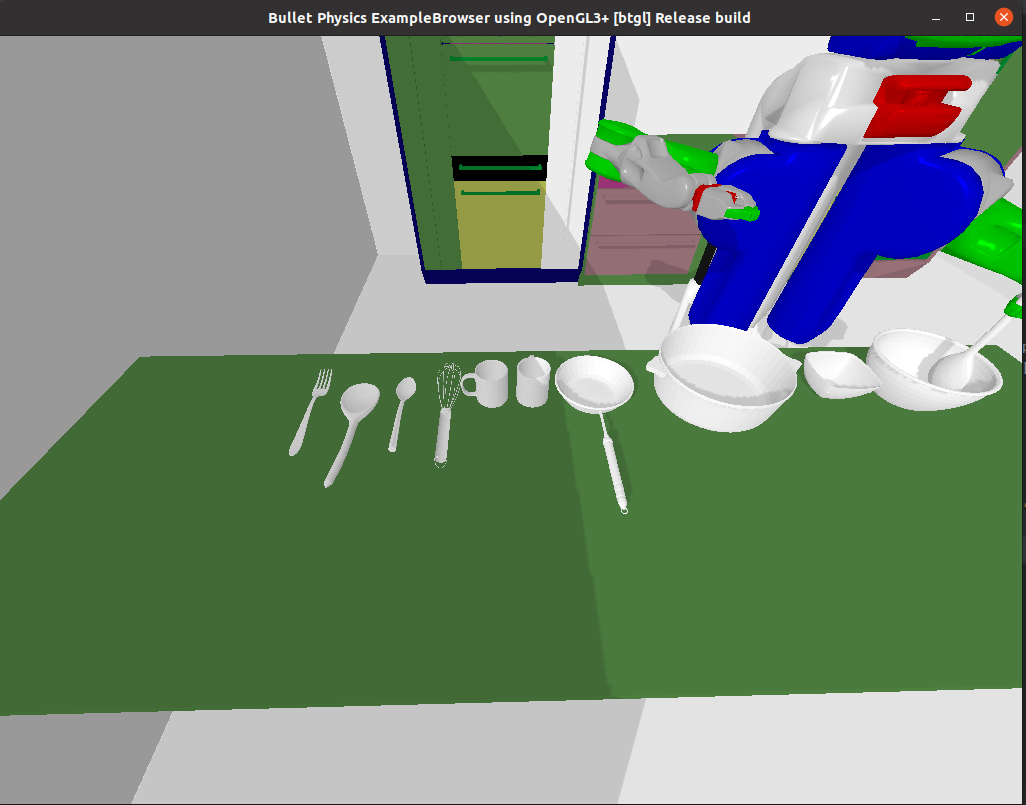
\includegraphics[scale=0.35]{Graphics/toolscontainersmodels.png}
    \label{fig:toolscontainersmodels}
    \caption{Used models for the simulation: \textit{Fork, WoodenSpoon, Spoon, Whisk, Mug, Cup, Pan, Pot, Small Bowl, Big Bowl}}
\end{figure}

PyCram bietet schon eine betrachtliche Anzahl an implementierten Aktionen, womit der Roboter manevriert werden kann. 
Unter diesen Aktionen befinden sich notwendige Navigationaktionen, sowie manipulative Aktionen wie Greifen und Platzieren. 
Außerdem bietet PyCram schon Schnittstellen bereit womit die Joints des Roboters bewegt werden können, diese Funktionen heißen dann zum Beispiel moveTorso().
BILDER CODE FUNKtIONEN

\section*{HIER STELLEN WIR UNSERE MOTIONS VOR}
Hier Vanessa fragen, wie wir ihre Motion referenzieren sollen, einfahc sagen es war vorhanden oder es detaillierten angeben?

\section*{Simulation to RealWorld gap}
\begin{itemize}
	\item Big Problem: Uncertaininty
	\item Perception Solution as first approach: RoboKudo
	\item Data acquisition: Blenderproc
	\item Model Training: YoloV8
	\item Results showing the real world Perception.
\end{itemize}